\section{How to Create Plots?}

We will now show several possibilities for plotting, using different
technologies. For each of the following technologies, we give an example to
provide an idea to the reader of how the work with this technology might look
like. The examples are in alphabetical order of the technology name; afterwards
we will only look closer into \texttt{pgfplots}.

\subsection{GNUplot}

\subsection{pgfplots}

\subsection{PSTricks}

\subsection{R and Sweave}

\toolname{R} is a well-known language for statistical computing and
graphics~\cite{Ihaka1998}.  A huge variety of modules is available at the
Comprehensive R Archive Network (CRAN)\footnote{%
  \href{https://cran.r-project.org}{https://cran.r-project.org}}.  One of these
modules is called \toolname{Sweave}, initially developed by Friedrich
Leisch~\cite{Leisch2002}.  It combines \LaTeX{} and \toolname{R} in the style of
literate programming—a concept developed by Donald E\@. Knuth~\cite{Knuth1992}.
A simple introduction was given by Uwe Ziegenhagen in his German article
\enquote{Datenanalyse mit Sweave, \LaTeX{} und R}~\cite{Ziegenhagen2010}.

In order to use \toolname{Sweave}, one needs to write a document like shown in
Listing~\ref{lst:sweave-example}.  By convention, the filename suffix is not
\texttt{*.tex} but \texttt{*.Snw}; this is important, because the \texttt{*.tex}
file will be create automatically.  A syntax highlighting mode is available for
the editor VIM\@.  After writing the file, one needs to start \toolname{R},
e.g., a \toolname{R} interactive shell.  With the command
\mintinline{R}{Sweave("filename.Snw")} the \toolname{R} code will be processed
and a \texttt{*.tex} file will be created, which can then be processed by, e.g.,
\hologo{pdfLaTeX}.

The example in Listing~\ref{lst:sweave-example} loads the exchange rates between
\euro{} and \$ from the homepage of the European Central Bank and plots it. The
output can be seen in Figure~\ref{fig:sweave-example}.

\begin{listing}[H]
  \inputminted{latex}{../examples/sweave-example.Snw}
  \caption{Plot the exchange rate between \euro{} and \$ dynamically using
    Sweave}
  \label{lst:sweave-example}
\end{listing}
\begin{figure}[!t]
  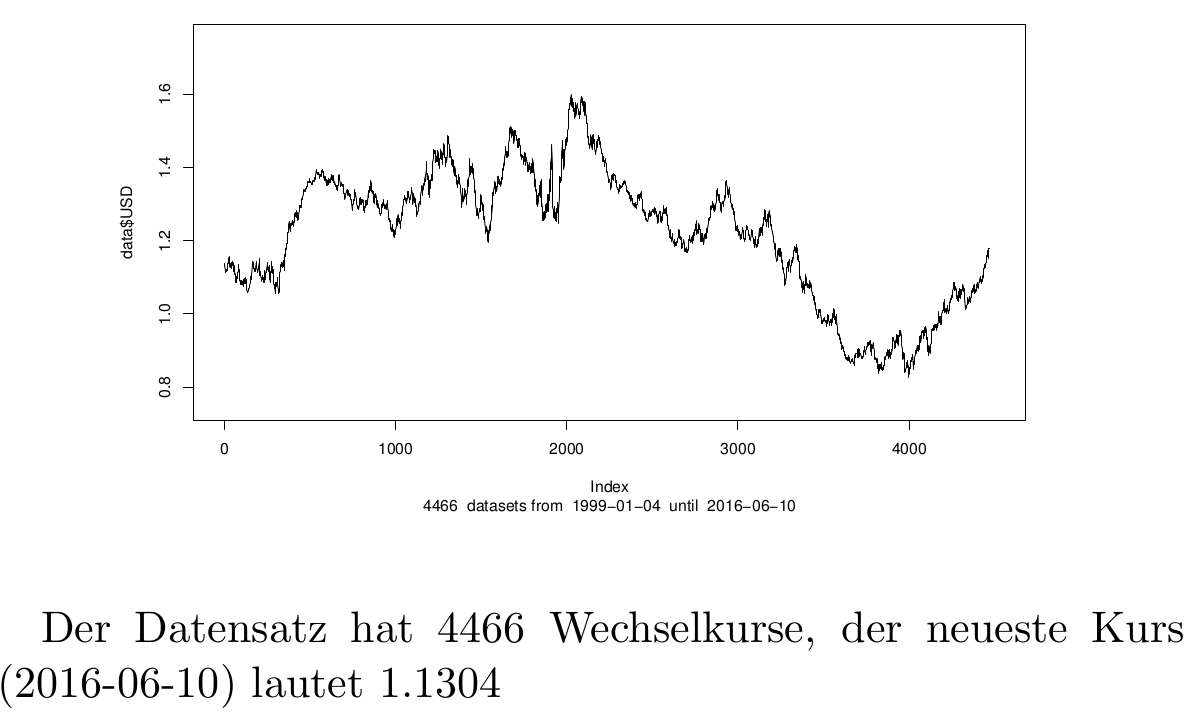
\includegraphics[width=\linewidth]{sweave-example}
  \caption{Screenshot of the Sweave example in Lst.~\ref{lst:sweave-example}}
  \label{fig:sweave-example}
\end{figure}
